\documentclass[tikz,border=4pt]{standalone}
\usepackage{ctex}
\usepackage{amsmath}
\usepackage{pgfplots}
\pgfplotsset{compat=1.18}

% p9-02a: 反比例函数几何意义——矩形面积=|k|
% 在曲线 y=6/x 上取点P(x,y)，作矩形，面积=xy=6=|k|
\begin{document}
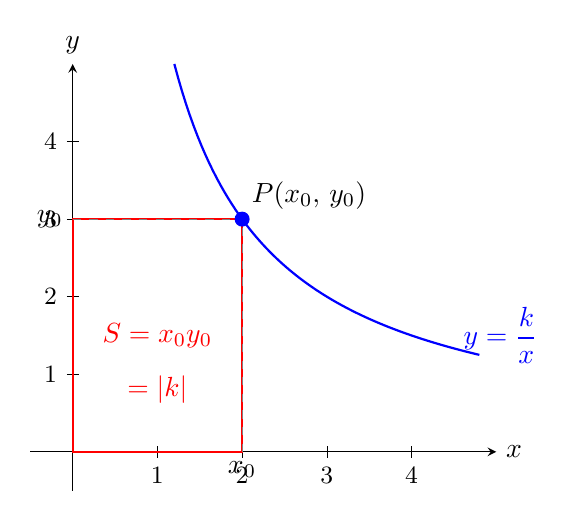
\begin{tikzpicture}
\begin{axis}[
  width=7.5cm, height=7cm,
  axis lines=center,
  xlabel={$x$}, ylabel={$y$},
  every axis x label/.style={at={(axis cs:5.0,0)}, anchor=west},
  every axis y label/.style={at={(axis cs:0,5.0)}, anchor=south},
  xmin=-0.5, xmax=5.0,
  ymin=-0.5, ymax=5.0,
  xtick={1,2,3,4},
  ytick={1,2,3,4},
  tick style={color=black},
  ticklabel style={font=\small},
  clip=false,
]
  % y = 6/x, 第一象限
  \addplot[blue, thick, domain=1.2:4.8, samples=80] {6/x};
  \node[right, blue] at (axis cs:4.5, 1.5) {$y=\dfrac{k}{x}$};

  % 取点 P(2, 3)
  \addplot[only marks, mark=*, mark size=2.5pt, blue] coordinates {(2,3)};
  \node[above right] at (axis cs:2,3) {$P(x_0,\,y_0)$};

  % 矩形（从原点到P的矩形）
  \draw[red, thick] (axis cs:0,0) rectangle (axis cs:2,3);
  % 面积标注
  \node[red] at (axis cs:1.0, 1.5) {$S = x_0 y_0$};
  \node[red] at (axis cs:1.0, 0.8) {$= |k|$};

  % 辅助虚线
  \draw[gray, dashed] (axis cs:2,0) -- (axis cs:2,3);
  \draw[gray, dashed] (axis cs:0,3) -- (axis cs:2,3);

  % 坐标标注
  \node[below] at (axis cs:2, 0) {$x_0$};
  \node[left] at (axis cs:0, 3) {$y_0$};
\end{axis}
\end{tikzpicture}
\end{document}
